\documentclass[11pt]{article}
\usepackage[margin=1in]{geometry}
\usepackage{amsmath,amssymb}
\usepackage{graphicx}
\usepackage{booktabs}
\usepackage{xcolor}
\usepackage{hyperref}

\newcommand{\E}{\mathbb{E}}
\newcommand{\code}[1]{\texttt{#1}}

\title{Process variance and PIT over time,\\ with and without bias correction}
\author{Claude}
\date{October 9, 2026}

\emergencystretch=3em
\begin{document}
\maketitle

\section*{Summary}

This note follows the learned process variance and the one-step-ahead PIT year by year,
to see whether the PIT flattens as the filter learns a smaller process variance. It is a
companion to \code{claude-forecast-width-10.8.26}, which explains why the forecasts are
too wide. It reaches four conclusions.

\begin{enumerate}
  \item \textbf{With bias correction, the process variance falls steadily, by 20--50 times by 2017.} The median
  falls from 0.61 in 1991 to 0.01 (GEDI) and 0.03 (LandTrendr). Without correction it levels off at
  0.1--0.25 after about 1995.
  \item \textbf{The PIT flattens only a little, and only for GEDI.} For GEDI heteroskedastic
  $R$ the PIT interquartile range (IQR) widens from 0.22 in 1995 to 0.28 by 2000 and then stays at 0.29--0.30
  (calibrated: 0.5). For LandTrendr it does not widen at all (about 0.15--0.21), even though the
  process variance falls nine-fold over the same years.
  \item \textbf{The bias correction centres the PIT; it does not flatten it.} Corrected, the mean and median
  PIT sit at about 0.54 in every year. Uncorrected they sit at about 0.27--0.36.
  \item \textbf{The process variance stops mattering after the first few years.} The process share of the forecast variance
  is already small by the mid-1990s, so the remaining width comes from the
  observation error $R$, as shown in the forecast-width note.
\end{enumerate}

%================================================================================
\section{Runs and definitions}

\begin{itemize}
  \item \textbf{Runs.} The two full grids, without the disturbance product (so no year is
  flagged), at all 538 sites, for each of the four observation-error models:
  \begin{itemize}
    \item uncorrected: \code{experiments/fullRunNoBias};
    \item bias-corrected: \code{experiments/fullRunBias}, with
    \code{bias = list(rho = 0.9, denom = "N", skip = 1)}.
  \end{itemize}
  Year $t$ runs from 1991 to 2017. Year 1990 is excluded because its forecast starts
  from the population-wide prior on the initial state.
  \item \textbf{Process variance $v_{t-1}$.} The posterior mean of the process variance after assimilating
  $y_{t-1}$:
  \[
    v_{t-1} = \E[1/\tau \mid y_{1:t-1}] = \sum_g \pi_{t-1}(g)/\tau_g ,
  \]
  where $\pi_{t-1}(g)$ is the posterior weight of grid point $\tau_g$ (\code{hist\$procVar} at
  $t-1$). This is the process variance used by the forecast of $y_t$, so it is plotted at year
  $t$, aligned with that year's PIT. (\code{claude-forecast-width-10.8.26} plots $v_t$, the
  same series one year later.)
  \item \textbf{PIT $u_t$.} The probability integral transform of $y_t$ under its one-step-ahead
  predictive: the predictive probability of a value $\le y_t$ (\code{hist\$pit}). If
  the predictive is calibrated, $u_t$ is uniform on $[0,1]$: mean and median 0.5,
  quartiles 0.25 and 0.75, IQR 0.5. An IQR below 0.5 means the
  PIT is concentrated in the middle, i.e.\ the predictive is too wide. A median away from 0.5
  means it is biased (below 0.5: forecasts too high).
  \item \textbf{Across-site summaries.} For each year, the median, IQR (25th--75th
  percentile) and mean over the 538 sites, of $v_{t-1}$ and of $u_t$.
  \item \textbf{Coverage error of the central 50\% interval.} The fraction of sites with
  $|2u_t - 1| \le 0.5$ (the observation falls in the predictive's central 50\% interval),
  minus 0.5. Positive values mean the forecast is too wide; 0 means calibrated.
  \item \textbf{Periods.} 1991--95, 1996--2000, 2001--05, 2006--11 and 2012--17, for the PIT
  histograms in Figure~\ref{fig:periods}.
\end{itemize}

%================================================================================
\section{Results}

\begin{figure}[p]
  \centering
  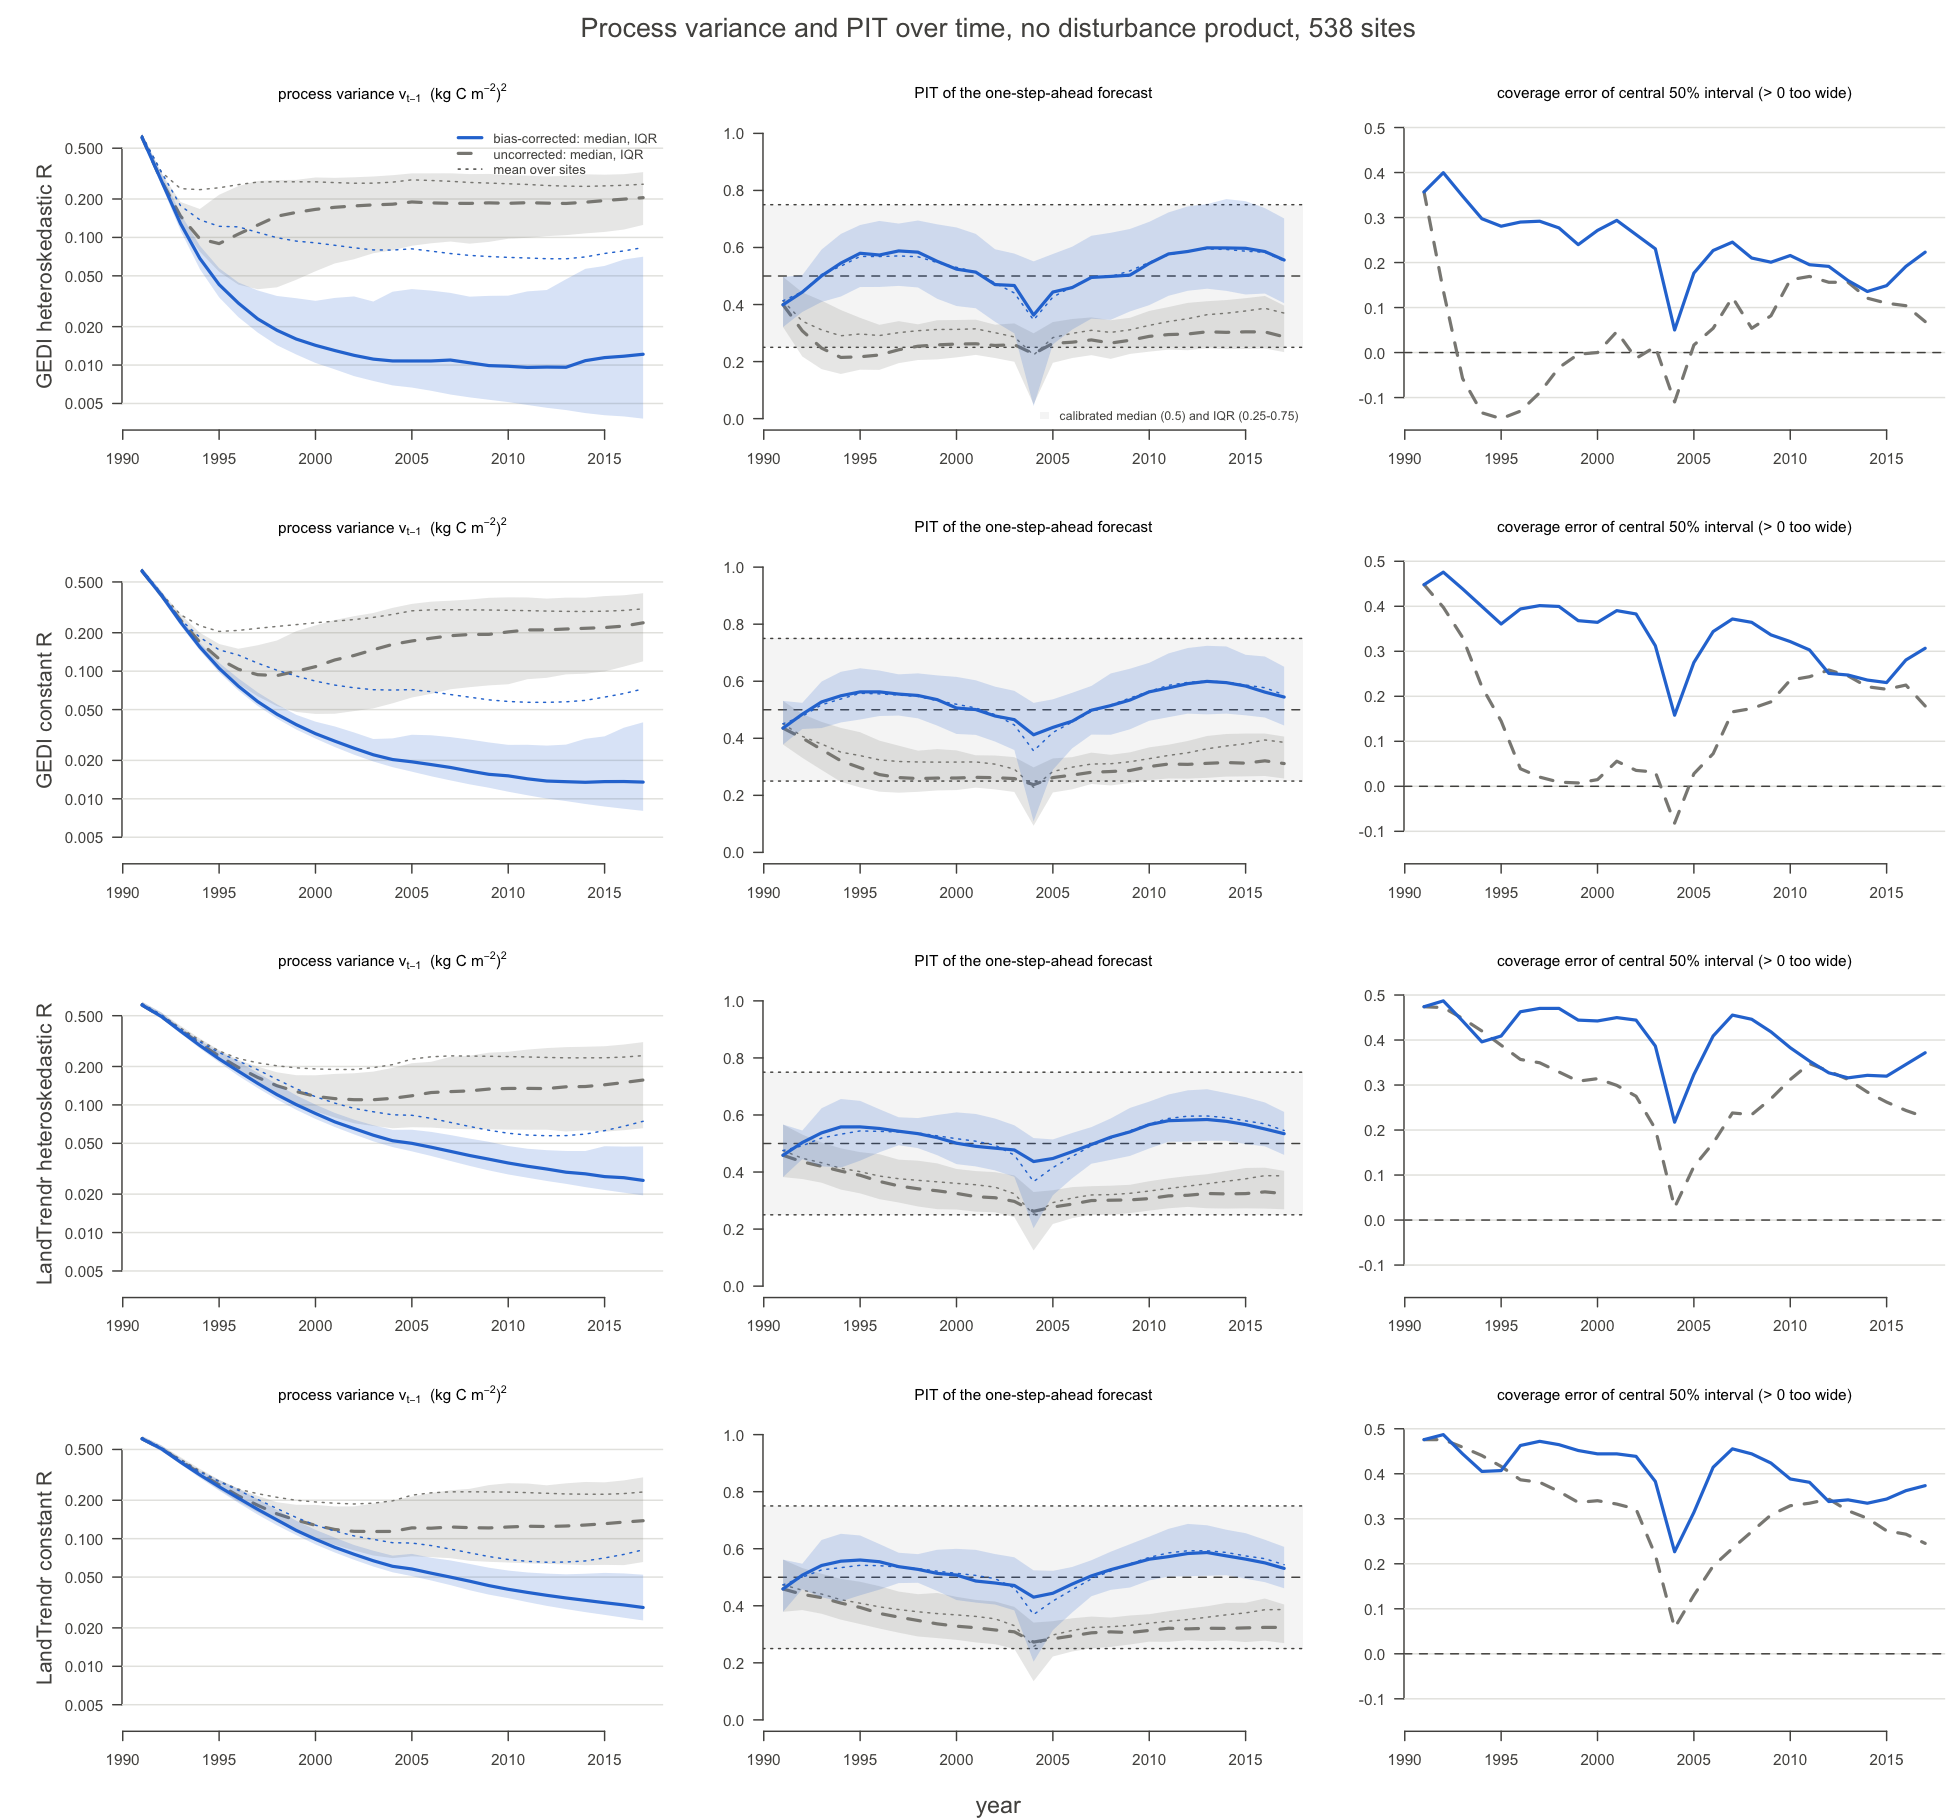
\includegraphics[width=\textwidth]{fw_pit_time.png}
  \caption{Per year, one row per observation-error model; blue = bias-corrected,
  gray dashed = uncorrected. \emph{Left:} process variance $v_{t-1}$ (log scale), median
  (thick line), IQR (band) and mean (dotted) over sites. \emph{Middle:} PIT $u_t$, median, IQR
  and mean over sites. The shaded strip and dotted lines at 0.25 and 0.75 are the calibrated
  quartiles. \emph{Right:} coverage error of the central 50\% interval.}
  \label{fig:time}
\end{figure}

\begin{figure}[p]
  \centering
  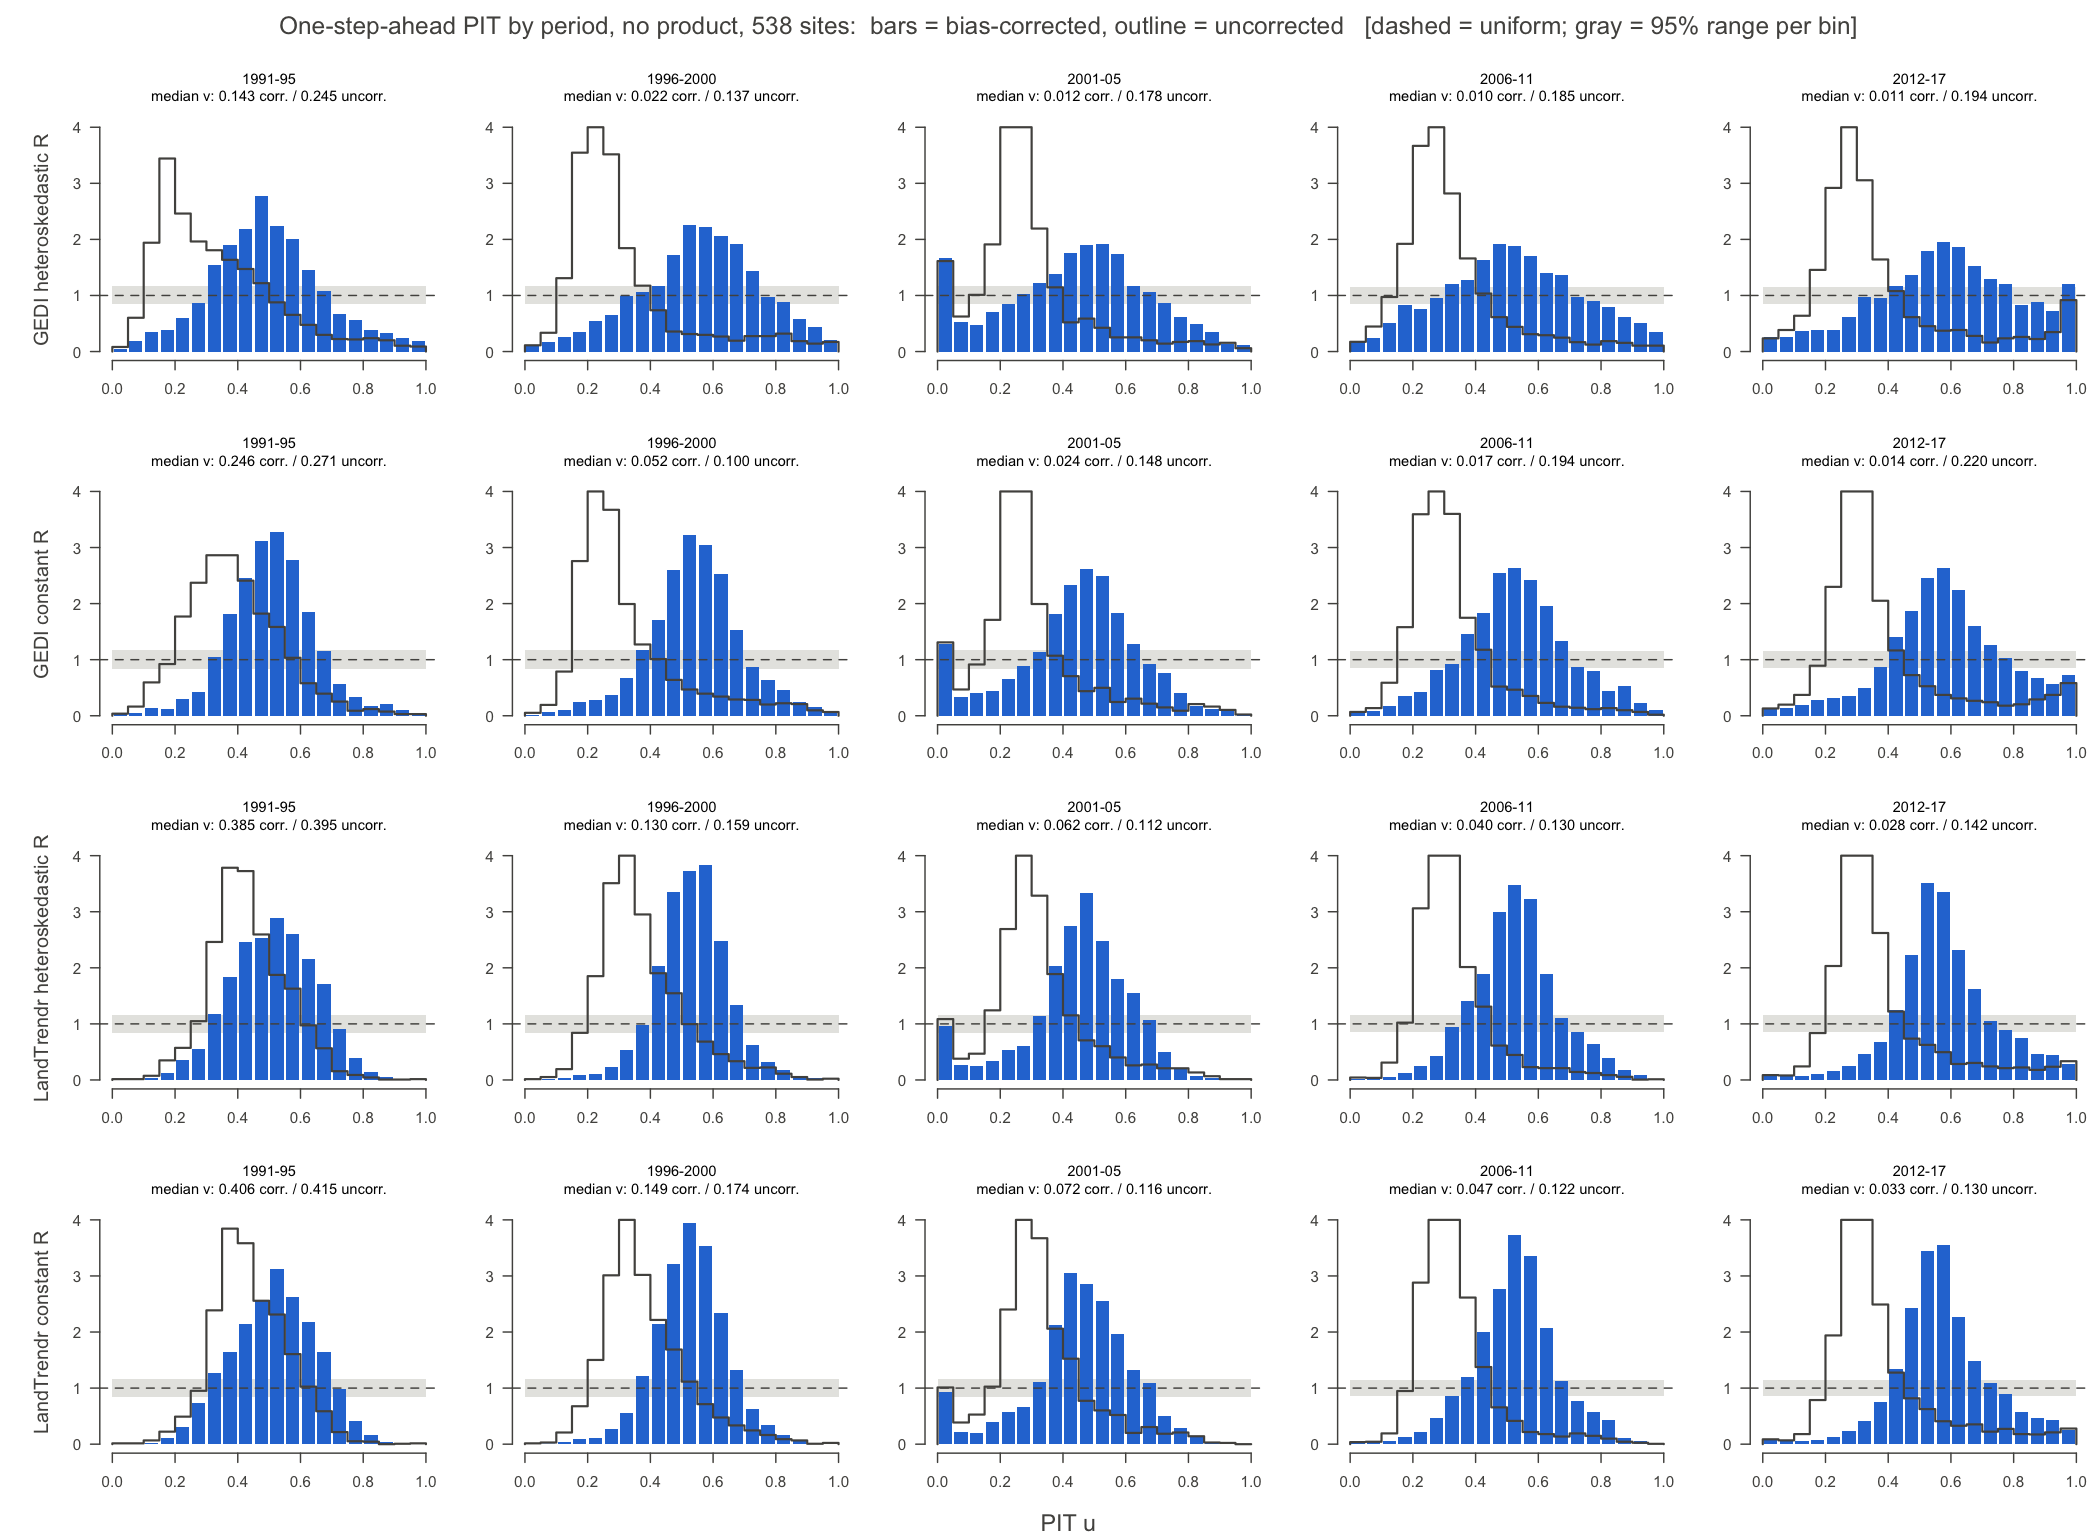
\includegraphics[width=\textwidth]{fw_pit_periods.png}
  \caption{PIT histograms by period (all sites and years in the period). Bars: bias-corrected;
  outline: uncorrected; dashed: uniform; gray: 95\% range of each bin under a uniform PIT.
  Panel titles give the median $v_{t-1}$ over the period.}
  \label{fig:periods}
\end{figure}

\begin{table}[ht]
  \centering\small
  \begin{tabular}{llrrrrrrr}
    \toprule
    & & \multicolumn{3}{c}{$v_{t-1}$} & \multicolumn{4}{c}{PIT $u_t$} \\
    \cmidrule(lr){3-5} \cmidrule(lr){6-9}
    model & year & median & IQR & mean & median & IQR & IQR width & cov.\ err.\ 50\% \\
    \midrule
    GEDI het.        & 1991 & 0.607 & 0.583--0.653 & 0.627 & 0.40 & 0.32--0.50 & 0.18 & 0.36 \\
                     & 1995 & 0.043 & 0.034--0.057 & 0.122 & 0.58 & 0.46--0.68 & 0.22 & 0.28 \\
                     & 2000 & 0.014 & 0.010--0.032 & 0.091 & 0.52 & 0.40--0.67 & 0.28 & 0.27 \\
                     & 2010 & 0.010 & 0.005--0.035 & 0.070 & 0.54 & 0.40--0.69 & 0.29 & 0.22 \\
                     & 2017 & 0.012 & 0.004--0.071 & 0.083 & 0.56 & 0.40--0.70 & 0.30 & 0.22 \\
    \addlinespace
    GEDI const.      & 1995 & 0.105 & 0.098--0.116 & 0.147 & 0.56 & 0.47--0.65 & 0.18 & 0.36 \\
                     & 2000 & 0.032 & 0.030--0.040 & 0.084 & 0.51 & 0.42--0.62 & 0.20 & 0.36 \\
                     & 2017 & 0.014 & 0.008--0.040 & 0.073 & 0.55 & 0.45--0.65 & 0.21 & 0.31 \\
    \addlinespace
    LandTrendr het.  & 1995 & 0.229 & 0.216--0.262 & 0.257 & 0.56 & 0.44--0.65 & 0.21 & 0.41 \\
                     & 2000 & 0.086 & 0.078--0.101 & 0.116 & 0.50 & 0.43--0.61 & 0.18 & 0.44 \\
                     & 2017 & 0.026 & 0.020--0.047 & 0.074 & 0.53 & 0.46--0.61 & 0.15 & 0.37 \\
    \addlinespace
    LandTrendr const.& 1995 & 0.255 & 0.238--0.288 & 0.280 & 0.56 & 0.44--0.65 & 0.21 & 0.41 \\
                     & 2000 & 0.099 & 0.090--0.117 & 0.128 & 0.51 & 0.42--0.60 & 0.18 & 0.44 \\
                     & 2017 & 0.029 & 0.023--0.052 & 0.082 & 0.53 & 0.46--0.61 & 0.15 & 0.37 \\
    \bottomrule
  \end{tabular}
  \caption{Bias-corrected runs, selected years: process variance $v_{t-1}$
  ((kg\,C\,m$^{-2}$)$^2$) and PIT over the 538 sites. Calibrated PIT: median 0.5, IQR
  0.25--0.75 (width 0.5), coverage error 0. Every year is in \code{fw\_pit\_time.csv}.}
  \label{tab:years}
\end{table}

\paragraph{Process variance (Figure~\ref{fig:time}, left).}
\begin{itemize}
  \item \textbf{With correction it keeps falling.} The median falls fastest in the first five
  years and keeps falling slowly after that. For GEDI it reaches about 0.01, for LandTrendr about 0.03 by 2017.
  \item \textbf{Without correction it levels off.} After about 1995 the uncorrected median stays at 0.1--0.25, and for GEDI it creeps up:
  the filter uses process variance to absorb the forecast bias (as in the forecast-width note).
  \item \textbf{The mean is much larger than the median and levels off at 0.06--0.13 after 2000.} The distribution
  over sites is right-skewed: most sites learn a small process variance, and a minority with
  large year-to-year jumps learn a much larger one. For GEDI heteroskedastic $R$ the upper
  quartile rises again after about 2013 (0.035 to 0.071), from sites whose biomass changes
  quickly late in the record.
\end{itemize}

\paragraph{PIT (Figure~\ref{fig:time}, middle and right; Figure~\ref{fig:periods}).}
\begin{itemize}
  \item \textbf{Centring: the correction works in every year.} Averaged over 1996--2017
  (excluding 2003--04, see below), the corrected mean PIT is 0.54 for every model.
  Uncorrected it is 0.33--0.36, with median 0.27--0.32: the uncorrected forecasts are too high
  throughout. The remaining 0.04 above 0.5 is the low disturbance tail of the predictive
  (forecast-width note, Section 3).
  \item \textbf{Concentration: the PIT flattens only a little, and only for GEDI.} For GEDI heteroskedastic $R$,
  the PIT IQR widens from 0.22 (1995) to 0.28 (2000) and then stays at 0.29--0.30, while
  the median $v_{t-1}$ falls only from 0.014 to 0.010. The central 50\% interval goes from 28 to 22
  points too wide. For GEDI constant $R$ the IQR stays at 0.18--0.21. For LandTrendr it
  \emph{narrows} slightly (0.21 to 0.15) even though $v_{t-1}$ falls nine-fold: the forecast
  errors shrink over time faster than the forecast variance, which stays dominated by $R$. In
  Figure~\ref{fig:periods} the corrected histograms stay humped in every period.
  \item \textbf{The uncorrected PIT can look better, by accident.} The uncorrected 50\% coverage error is near 0 or
  even negative for GEDI in 1995--2005. That is not calibration: the bias pushes the
  observations away from the centre of a predictive that is too wide, and the two errors partly cancel.
  The uncorrected PIT IQR is in fact narrower (0.13--0.15) than the corrected one.
  \item \textbf{2003--04 is a disturbance year.} Many sites lose biomass in 2003--04, which
  the undisturbed forecast does not expect. The PIT drops (median 0.36--0.44 corrected), its
  lower quartile falls to 0.04--0.20, and the coverage error dips. This is real disturbance,
  not better calibration, so it is excluded from the averages above.
  \item \textbf{A late tail toward high PIT.} From about 2010 the corrected GEDI histograms grow a tail toward
  $u_t = 1$, i.e.\ forecasts that are too low at some sites. This matches the regrowth
  over-correction seen at site 300: $b$ is learned in mature stands and is too negative for
  regrowing stands.
\end{itemize}

\paragraph{Interpretation.}
The process variance is the only part of the predictive variance that the filter learns,
and it does shrink. But after the first few years it is a small part of the predictive
variance (a median share of 1--4\% of the full predictive variance from 1996 on, against 17--83\% for $R$;
see \code{fw\_pit\_time.csv} and the forecast-width note). Once it is small, shrinking it further
cannot flatten the PIT. In the R-scaling experiment (\code{rs\_pit.png}), reducing $R$
flattens the PIT. That points to the observation-error model, not the process variance, as
the thing to change.

%================================================================================
\section*{Reproducing}

\code{Rscript claude-working-docs/forecast\_width\_analysis.R} (section 6), from the
repository root, with \code{EXP\_DIR} set if the experiment folders are elsewhere. It writes
\code{fw\_pit\_time.png}, \code{fw\_pit\_periods.png} and the per-year table
\code{fw\_pit\_time.csv}.

\end{document}
